\documentclass [10pt]{article}
\textheight	8.7in
\textwidth	6.5in
\topmargin	    0in
\oddsidemargin  0in
\evensidemargin 0in
\baselineskip 15pt

\usepackage{amssymb,amsmath,amstext}
\usepackage{amsfonts}
\usepackage{mathtools}
\usepackage{tikz}
\usetikzlibrary{automata,arrows,calc,positioning}

\begin{document}
\title{Theory of Computation Assignment no. 2}
\author{Goktug Saatcioglu}
\date{}
\maketitle
\begin{enumerate}
	\item[\textbf{(1)}]
	\begin{enumerate}
		\item[i.]
		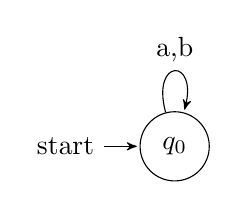
\begin{tikzpicture}[baseline=(q_0.north),>=stealth',shorten >=1pt, auto,node distance=1cm,align=center]
			\node[state,initial] (q_0) {$q_0$};
			\path[->]
			(q_0) edge [loop above] node {a,b} ();
		\end{tikzpicture}
		\\Where $q_{0} = \emptyset$ (the empty set).
		\item[ii.]
		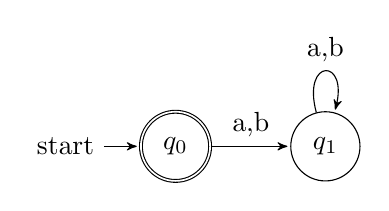
\begin{tikzpicture}[baseline=(q_0.north),>=stealth',shorten >=1pt, auto,node distance=1cm,align=center]
			\node[state,initial,accepting] (q_0) {$q_0$};
			\node[state] [right= of q_0] (q_1)  {$q_1$};
			\path[->]
			(q_0) edge node {a,b} (q_1)
			(q_1) edge [loop above] node {a,b} ();
		\end{tikzpicture}
		\\Where $q_{0} = \lambda$ (the empty string) and $q_{1} \ne \lambda$ (anything but the empty string). 
		\item[iii.]
		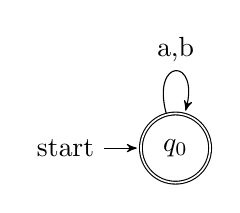
\begin{tikzpicture}[baseline=(q_0.north),>=stealth',shorten >=1pt, auto,node distance=1cm,align=center]
			\node[state,initial,accepting] (q_0) {$q_0$};
			\path[->]
			(q_0) edge [loop above] node {a,b} ();
		\end{tikzpicture}
		\\Where $q_{0} \in \Sigma^{*}$ (the set of all strings).
	\end{enumerate}
	\item[\textbf{(2)}]
	\begin{enumerate}
		\item[viii.]
		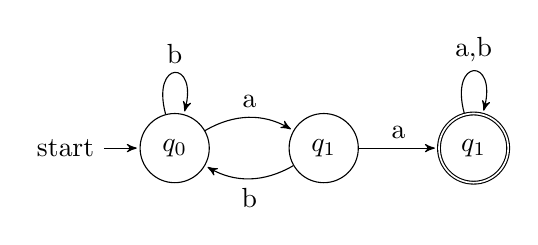
\begin{tikzpicture}[baseline=(q_0.north),>=stealth',shorten >=1pt, auto,node distance=1cm,align=center]
			\node[state,initial] (q_0) {$q_0$};
			\node[state] [right= of q_0] (q_1) {$q_1$};
			\node[state,accepting] [right= of q_1] (q_2) {$q_1$};
			\path[->]
			(q_0) edge [loop above] node {b} ()
			(q_0) edge [bend left] node {a} (q_1)
			(q_1) edge [bend left] node {b} (q_0)
			(q_1) edge node {a} (q_2)
			(q_2) edge [loop above] node {a,b} ();
		\end{tikzpicture}
		\\Where $q_{0} \in \Sigma^{*}$ (the set of all strings), $q_{1} \in \Sigma^{*}_{a}$ (the set of all strings containing $a$ as a substring) and $q_{1} \in \Sigma^{*}_{aa}$ (the set of all strings containing $aa$ as a substring).
		\item[xii.]
		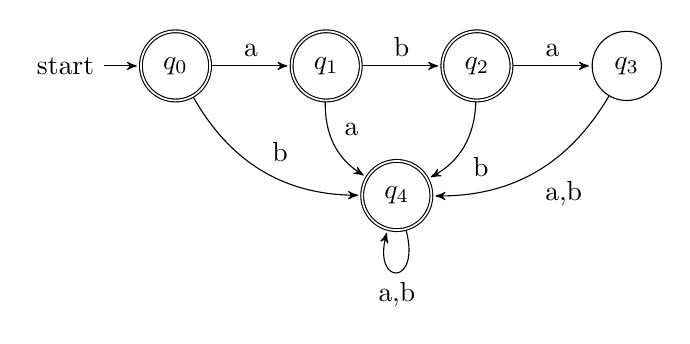
\begin{tikzpicture}[baseline=(q_0.north),>=stealth',shorten >=1pt, auto,node distance=1cm,align=center]
			\node[state,initial,accepting] (q_0) {$q_0$};
			\node[state,accepting] [right= of q_0] (q_1) {$q_1$}; 
			\node[state,accepting] [right= of q_1] (q_2) {$q_2$};
			\node[state] [right= of q_2] (q_3) {$q_3$};
			\node[state,accepting] [below right=1cm and 0.25cm of q_1] (q_4) {$q_4$};
			\path[->]
			(q_0) edge [bend right] node {b} (q_4)
			(q_0) edge node {a} (q_1)
			(q_1) edge [bend right] node {a} (q_4)
			(q_1) edge node {b} (q_2)
			(q_2) edge [bend left] node {b} (q_4)
			(q_2) edge node {a} (q_3)
			(q_3) edge [bend left] node {a,b} (q_4)
			(q_4) edge [loop below] node {a,b} ();
		\end{tikzpicture}
		\\Where $q_0 = q_1 = q_2 = q_4 = \{w|w \in \Sigma^{*}, w \ne aba\}$ (the set of all strings excepting $aba$) and $q_3 = aba$ (the $aba$ string).
		\item[xiv.]
		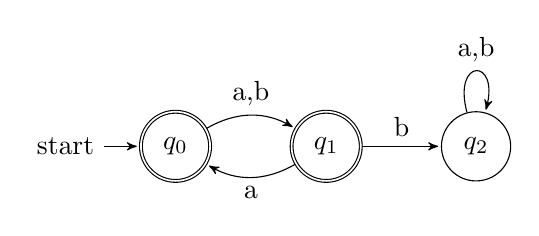
\begin{tikzpicture}[baseline=(q_0.north),>=stealth',shorten >=1pt, auto,node distance=1cm,align=center]
			\node[state,initial,accepting] (q_0) {$q_0$};
			\node[state,accepting] [right= of q_0] (q_1) {$q_1$};
			\node[state] [right= of q_1] (q_2) {$q_2$};
			\path[->]
			(q_0) edge [bend left] node {a,b} (q_1)
			(q_1) edge [bend left] node {a} (q_0)
			(q_1) edge node {b} (q_2)
			(q_2) edge [loop above] node {a,b} (); 
		\end{tikzpicture}
		\\Let the set of all strings with $a$'’s in all the even positions and $a$'’s or $b$’'s in the odd positions be named $VALID$. Any other set that is not $VALID$ is $INVALID$. Thus, $q_0 = q_1 = VALID$ and $q_2 = INVALID$.
	\end{enumerate}
	\item[\textbf{(3)}]Let $M_{A}$ and $M_{B}$ be DFA's that recognize the languages $A$ and $B$ respectively, and assume that $M_{A}=(\Sigma,Q_{A},q_{A},F_{A},\delta_{A})$ and $M_{B}=(\Sigma,Q_{B},q_{B},F_{B},\delta_{B})$. Then the formal definition of an automaton $M_{A\Delta B} = (\Sigma,Q_{A\Delta B},q_{A\Delta B},F_{A\Delta B},\delta_{A\Delta B})$, where $A\Delta B = (A\setminus B)\cup(B\setminus A)$, is as follows.
	\begin{align}
		Q_{A\Delta B} &\coloneqq Q_{A} \times Q_{B} \nonumber \\
		q_{A\Delta B} &\coloneqq (q_{A},q_{B}) \nonumber \\
		F_{A\Delta B} &\coloneqq \{(q,p)|(q\in F_{A} \land p\notin F_{B})\lor(q\notin F_{A} \land p\in F_{B})\} && \text{where $(q,p) \in Q_{A\Delta B}$} \nonumber \\
		&= (F_{A}\times (Q_{B}\setminus F_{B}))\cup((Q_{A}\setminus F_{A})\times F_{B}) \nonumber \\
		\delta_{A\Delta B} &\coloneqq Q_{A\Delta B} \times \Sigma \rightarrow Q_{A\Delta B} \nonumber \\
		&\implies \delta_{A\Delta B}((q,p),w) = (\delta_{A}(q,w),\delta_{B}(p,w)) && \text{where $(q,p) \in Q_{A\Delta B}$, $w\in \Sigma$} \nonumber 
	\end{align}
	\item[\textbf{(4)}]Let $M=(\Sigma,Q,q,F,\delta)$ be a DFA. We prove that for any two words $u,v \in \Sigma^{*}$ and any state $q \in Q$ that $\delta^{*}(q,uv)=\delta^{*}(\delta^{*}(q,u),v)$, where $uv$ denotes the concatentation of $u$ and $v$ and $\left| v \right| = n$ where $n \ge 0$, using induction.\\
	\textbf{Base case.} $n = 0 \implies \left|v\right| = 0 \implies v = \lambda$.
	\begin{align}
	\label{1} \tag{1} \forall p \in Q \quad \delta^{*}(p,\lambda) &= p\\
	\delta^{*}(q,uv)&=\delta^{*}(q,u\lambda) \nonumber \\
	&=\delta^{*}(q,u) \nonumber \\
	&=\delta^{*}(\delta^{*}(q,u),\lambda) && \text{using property \ref{1}} \nonumber \\ 
	&\therefore \text{holds true for base case} \nonumber
	\end{align}
	Since the LHS $=$ RHS the base case holds.\\
	\textbf{Inductive step.} For some $n \ge 0$, assume that $\delta^{*}(q,uv) = \delta^{*}(\delta^{*}(q,u),v)$ when $\left|v\right| = n$. Now for $k = n$, consider a $v'$ such that $\left|v'\right| = k + 1$ and $v' = wa$, where $w \in \Sigma^{*}$ such that $\left|v\right| = l \le k + 1$ and $a \in \Sigma$. Now we evaluate $\delta^{*}(q,uv')$.
	\begin{align}
	\label{2} \tag{2} \forall p \in Q \quad \delta^{*}(p,wa) &= \delta(\delta^{*}(p,w),a) && \text{where $w \in \Sigma^{*}$ and $a \in \Sigma$}\\
	\delta^{*}(q,uv') &= \delta^{*}(q,uwa) && \text{$v' = wa$} \nonumber \\
	&= \delta(\delta^{*}(q,uw),a) && \text{using property \ref{2}} \nonumber \\
	&= \delta(\delta^{*}(\delta^{*}(q,u),w),a) && \text{by the induction hypothesis} \nonumber \\
	&= \delta^{*}(\delta^{*}(q,u),wa) && \text{using property \ref{2}} \nonumber \\
	\label{3} \tag{3} &= \delta^{*}(\delta^{*}(q,u),v') && \text{$wa = v'$}
	\end{align}
	\textbf{Conclusion.} By the principle of induction, we see that $\delta^{*}(q,uv) = \delta^{*}(\delta^{*}(q,u),v)$ for $\left| v \right| = n$ where $n \ge 0$. $\Box$
\end{enumerate}
\end{document}